\documentclass[12pt]{article}
\usepackage{amsmath}
\usepackage{listings}
\usepackage{enumerate}
\usepackage{color}
\usepackage{graphicx}
\usepackage[margin=0.5in]{geometry}
\title{Project 2}

\author{Dan Kolbman}
\date{October 20, 2014}

\definecolor{mygreen}{rgb}{0,0.6,0}
\definecolor{mygray}{rgb}{0.95,0.95,0.95}
\definecolor{mymauve}{rgb}{0.58,0,0.82}
%\definecolor{mygray}{RGB}{22, 22, 22}}

\lstset{ %
  language=Python,
  backgroundcolor=\color{mygray},   % choose the background color
  basicstyle=\footnotesize,        % size of fonts used for the code
  breaklines=true,                 % automatic line breaking only at whitespace
  captionpos=b,                    % sets the caption-position to bottom
  commentstyle=\color{mygreen},    % comment style
  %escapeinside={\%*}{*)},          % if you want to add LaTeX within your code
  keywordstyle=\color{blue},       % keyword style
  stringstyle=\color{mymauve},     % string literal style
  frame=L,
  xleftmargin=\parindent,
  showstringspaces=false
}
\begin{document}
  
  \maketitle

  \section{Interpolation of Reflector Points}
  A cubic spline was used to interpolate given points on the reflector surface.
  The first derivatives of the $y_1$ and $y_n$ points were used to apply
  clamped boundary conditions to the spline.
  The derivative of the last knot, $y_5\prime$, was doubled to show its effects
  on the complete spline. Only the interpolated line between the last 3 knots
  $y_3$ and $y_5$ were visibly affected by changing the boundary condition.
  Overall, using a cubic spline for interpolation yielded very good results.

  \begin{figure}[h!]
    \centering
    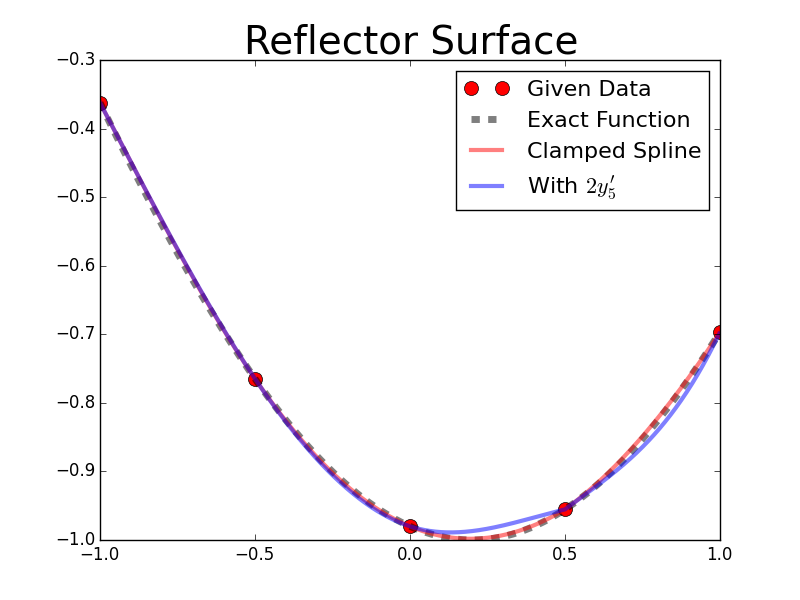
\includegraphics[scale=0.9]{cos.png}
    \caption{Fits for $f(x)=-cos(x-0.2)$}
  \end{figure}

  \begin{figure}[h!]
    \centering
    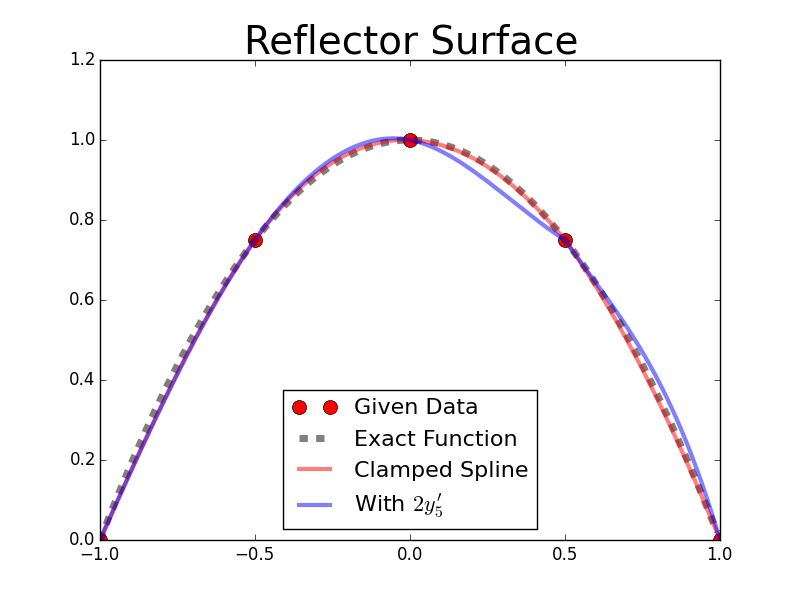
\includegraphics[scale=0.75]{parabola.png}
    \caption{Fits for $f(x)=1-x^2$}
  \end{figure}

  \begin{figure}[h!]
    \centering
    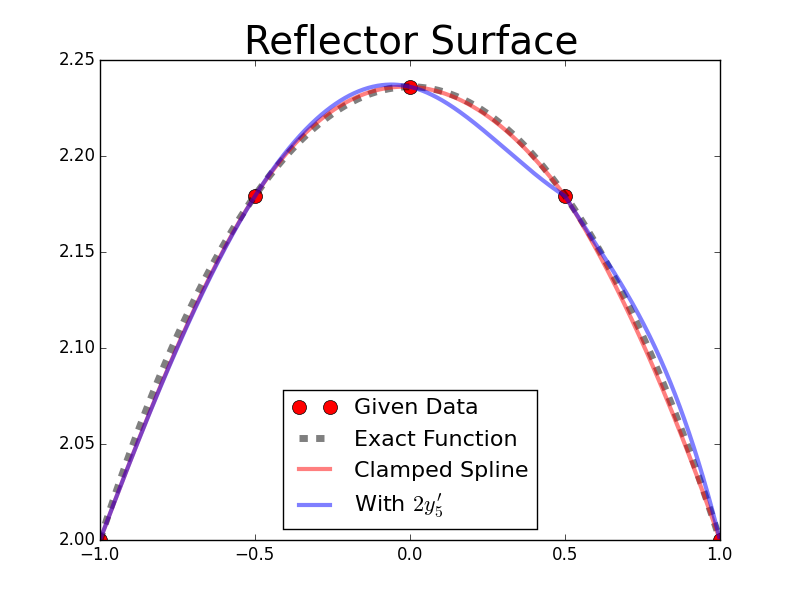
\includegraphics[scale=0.75]{arc.png}
    \caption{Fits for $f(x)=\sqrt{5-x^2}$}
  \end{figure}

  \clearpage

  \section{Error Analysis}
  Error was calculated using the root mean square error (Eq \ref{eq:rmse}) on
  all interpolated points.
  \begin{equation}
    \label{eq:rmse}
    RMSE = \sqrt{\frac{\sum_{i=1}^n(\hat{y}_i-y_i)^2}{n}}
  \end{equation}

  Doubling the derivative of the last knot resulted in a worse fit, as expected.
 
  \begin{table}[h!]
  \centering
  \begin{tabular}{| c | c | c |}
    \hline
    $f(x)$         & RMSE ($y_5^\prime$) & RMSE ($2y_5^\prime$)\\ \hline
    $-cos(x-0.2)$  & 0.00357 & 0.00963    \\
    $1-x^2$        & 0.01047 & 0.02846    \\
    $\sqrt{5-x^2}$ & 0.00295 & 0.00697    \\ \hline
  \end{tabular}
  \end{table}


  \section{Derivatives}

  The derivative of the interpolated spline was found using a central difference
  finite difference. Its accuracy largely depends on the resolution available
  from the spline. These results come from a spline with 200 points for each
  segment, or 800 total points.
  The error is expected te be atleast as bad as the function itself as new
  error will be introduced from the numerical derivative. It also must be worse
  as there were less conditions met for the derivative (2) than the function (5).
  Evaluating the error in the form of the RMSE reveals this is true.

  \centering
  \begin{tabular}{| c | c | c |}
    \hline
    $f(x)$         & $f^\prime(x)$             & RMSE     \\ \hline
    $-cos(x-0.2)$  & $-sin(0.2-x)$             & 0.02398    \\
    $1-x^2$        & $-2x$                     & 0.07096   \\
    $\sqrt{5-x^2}$ & $\frac{-x}{\sqrt{5-x^2}}$ & 0.01971    \\ \hline
  \end{tabular}

  \begin{figure}[h!]
    \centering
    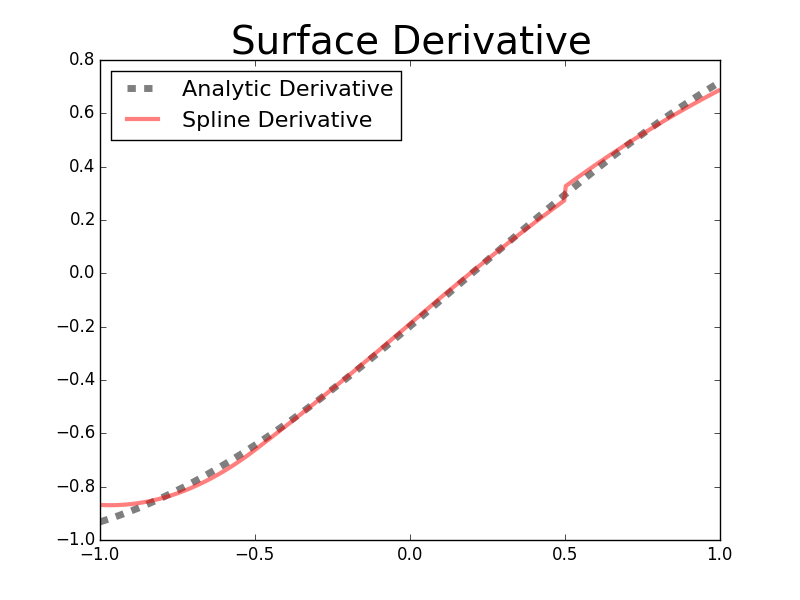
\includegraphics[scale=0.75]{cosderiv.png}
    \caption{Fits for $f^\prime(x)=-sin(0.2-x)$}
  \end{figure}

  \begin{figure}[h!]
    \centering
    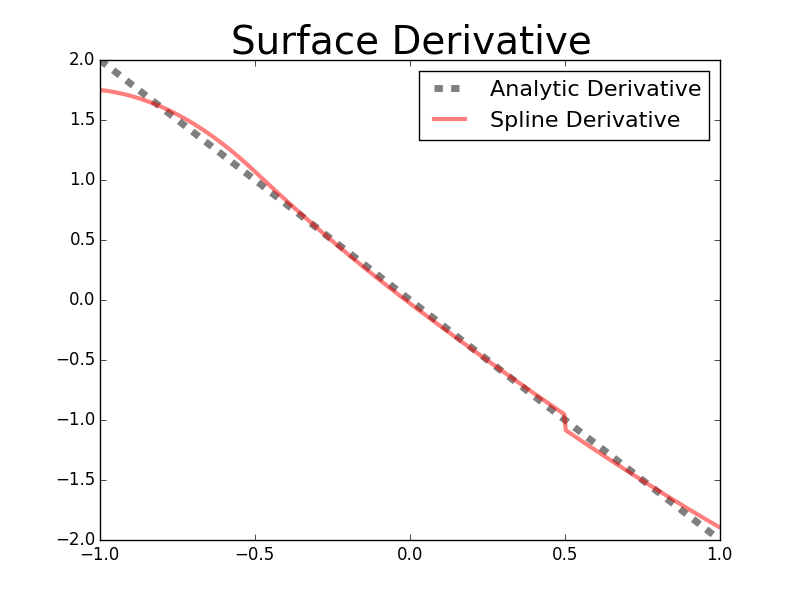
\includegraphics[scale=0.75]{pderiv.png}
    \caption{Fits for $f^\prime(x)=-2x$}
  \end{figure}

  \begin{figure}[h!]
    \centering
    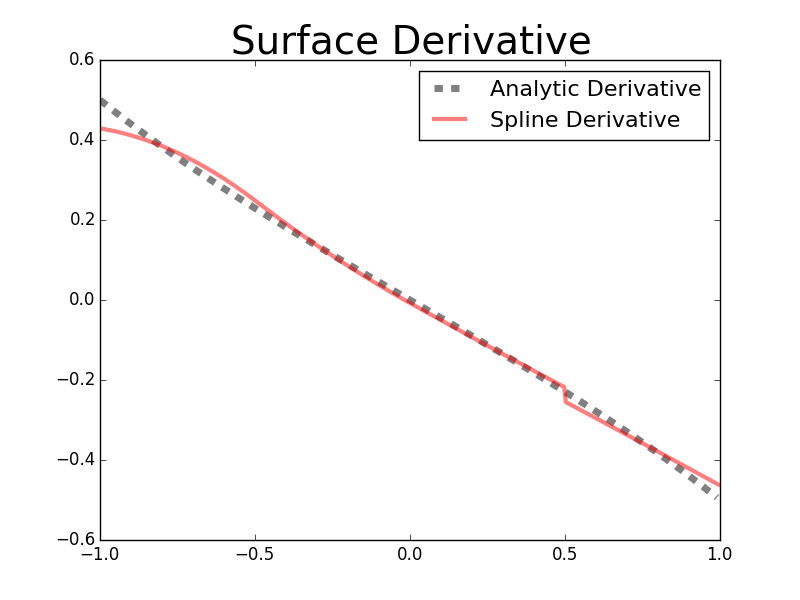
\includegraphics[scale=0.75]{arcderiv.png}
    \caption{Fits for $f^\prime(x)=\frac{-x}{\sqrt{5-x^2}}$}
  \end{figure}
  
\end{document}
